% Prepared from the final Word manuscript, 7 November 2026.
% Official Springer Nature authoring class; pdfLaTeX; no line numbers.
\documentclass[pdflatex,sn-basic,Numbered]{sn-jnl}
\usepackage[T1]{fontenc}
\usepackage[utf8]{inputenc}
\usepackage{amsmath,amssymb,mathtools}
\usepackage{xcolor}
\usepackage{graphicx,longtable,booktabs,array,calc,multirow}
\usepackage{adjustbox}
\usepackage{microtype}
\usepackage{xurl}
\usepackage{fancyvrb}
\usepackage{caption}
\usepackage{placeins}
\usepackage{etoolbox}
\usepackage{bookmark}
\captionsetup{labelsep=space,labelfont=bf,font=small}
\captionsetup[figure]{name=Fig.}
\captionsetup[table]{name=Table}
\setcounter{secnumdepth}{3}
\setlength{\emergencystretch}{2em}
\urlstyle{same}
\hypersetup{hidelinks,pdftitle={Direct cognition problem: a semantic skeleton of mathematics and its growth},pdfauthor={Vasilii A. Gromov; Nikolai N. Evdokimov}}
\newcommand{\tightlist}{\setlength{\itemsep}{0pt}\setlength{\parskip}{0pt}}
\newcommand{\passthrough}[1]{#1}
\newsavebox{\displaybox}
\newcommand{\fitdisplay}[1]{\sbox{\displaybox}{$\displaystyle #1$}\ifdim\wd\displaybox>\linewidth\resizebox{\linewidth}{!}{\usebox{\displaybox}}\else\usebox{\displaybox}\fi}
\makeatletter
\newsavebox\pandoc@box
\newcommand*\pandocbounded[1]{\sbox\pandoc@box{#1}\ifdim\wd\pandoc@box>\linewidth\resizebox{\linewidth}{!}{\usebox\pandoc@box}\else\usebox\pandoc@box\fi}
\patchcmd\longtable{\par}{\if@noskipsec\mbox{}\fi\par}{}{}
\makeatother
\raggedbottom
\renewcommand{\thetable}{S\arabic{table}}
\renewcommand{\thefigure}{S\arabic{figure}}
\begin{document}
\title[A semantic skeleton of formal knowledge]{Direct cognition problem: a semantic skeleton of mathematics and its growth}
\subtitle{Supporting appendices}
\author[1]{\fnm{Vasilii A.} \sur{Gromov}}\email{stroller@rambler.ru}
\author*[1]{\fnm{Nikolai N.} \sur{Evdokimov}}\email{nevdokimov@hse.ru}
\affil[1]{\orgdiv{Laboratory for Semantic Analysis}, \orgname{National Research University Higher School of Economics}, \orgaddress{\street{11 Pokrovsky Bulvar}, \city{Moscow}, \postcode{109028}, \country{Russia}}}
\maketitle
\noindent\small ORCID (Nikolai N. Evdokimov): \url{https://orcid.org/0009-0003-3756-8281}\par\normalsize

\section*{Appendix A. Combinatorial bounds and resources}\label{appendix-a.-combinatorial-bounds-and-resources}
\addcontentsline{toc}{section}{Appendix A. Combinatorial bounds and resources}

\subsection*{A.1. Resources and notation}\label{a.1.-resources-and-notation}
\addcontentsline{toc}{subsection}{A.1. Resources and notation}

Resource accounting distinguishes the active representation \(M_{S}\), reserve \(M_{P}\), archive \(M_{\Omega}\), and peak process memory. Moving a proof to disk does not discard knowledge. Equal numbers of anchors therefore imply neither equal certificate sizes nor equal memory use (Table S1).

\begingroup
\small
\setlength{\tabcolsep}{3pt}
\renewcommand{\arraystretch}{1.13}

\begin{longtable}[]{@{}
  >{\raggedright\arraybackslash}p{(\linewidth - 2\tabcolsep) * \real{0.1707}}
  >{\raggedright\arraybackslash}p{(\linewidth - 2\tabcolsep) * \real{0.8293}}@{}}
\caption{Notation, mathematical objects, and resource units}\label{tab:8}\tabularnewline
\toprule\noalign{}
\begin{minipage}[b]{\linewidth}\raggedright
\textbf{Notation}
\end{minipage} & \begin{minipage}[b]{\linewidth}\raggedright
\textbf{Object and unit}
\end{minipage} \\
\midrule\noalign{}
\endfirsthead
\toprule\noalign{}
\begin{minipage}[b]{\linewidth}\raggedright
\textbf{Notation}
\end{minipage} & \begin{minipage}[b]{\linewidth}\raggedright
\textbf{Object and unit}
\end{minipage} \\
\midrule\noalign{}
\endhead
\bottomrule\noalign{}
\endlastfoot
\(|F|_{AST}\) & Number of all syntax-tree vertices; metric for the main bounds \(L = 25,200\) \\
\(\ell_{leaf}(F)\) & Number of leaves; metric for the separate implicational KSP benchmark \\
\(H_{d}^{sch}\) & Canonical schemata through depth \(d\) under the declared constraints \\
\(H_{4}\) & Small exact schematic benchmark through depth 4, with every stored schema of size at most 25 \\
H14 & Name of an earlier configuration, not depth 14 or benchmark \(H_{4}\) \\
\(\Omega_{0},\Omega_{b}\) & Common initial archive and archive of a verified continuation \\
\end{longtable}

\endgroup

The relation between the two size metrics depends on the language. A purely implicational formula satisfies \(|F|_{AST} = 2\ell_{leaf}(F) - 1\), whereas negation or modality invalidates this equality. Budget \(b\) covers the declared computational scope; accounting records the historical cost of constructing \(\Omega_{0}\) separately.

\subsection*{A.2. Combinatorial costs and finite approximation}\label{a.2.-combinatorial-costs-and-finite-approximation}
\addcontentsline{toc}{subsection}{A.2. Combinatorial costs and finite approximation}

\subsubsection*{A.2.1. Number of potential pairs}\label{a.2.1.-number-of-potential-pairs}
\addcontentsline{toc}{subsubsection}{A.2.1. Number of potential pairs}

Two-premise modus ponens admits an exact count of potential pairs before filtering. Let \(V_{\leq d}\) contain the available formulae, \(F_{d}\) denote the new frontier, \(I_{\leq d}\) denote the implicational major premises, and \(F_{d}^{I} = F_{d} \cap I_{\leq d}\). Restricting attention to pairs with at least one new premise gives

\[\fitdisplay{P_{d} = |F_{d}|\,|I_{\leq d}| + |V_{< d}|\,|F_{d}^{I}|.}\]

The two terms divide the ordered pairs by premise role. The first term counts a new minor premise, including pairs with two new premises; the second counts a new major premise and an old minor premise. This equality describes Cartesian enumeration under that division of roles; structural indexing reduces actual checks, whereas other rules require their own counters.

The potential-pair count satisfies \(P_{d} \leq N_{d}^{2}\) for \(N_{d} = |V_{\leq d}|\). A single check also incurs costs for formula size, unification, and side conditions. The inequality thus bounds pairs, not the generator's total running time, and schemata with several matching results can produce more conclusions than their pair count alone suggests.

\subsubsection*{A.2.2. Exponential size of the explicit representation}\label{a.2.2.-exponential-size-of-the-explicit-representation}
\addcontentsline{toc}{subsubsection}{A.2.2. Exponential size of the explicit representation}

An explicit-space lower bound requires a precise vertex convention. In the following result, each vertex represents a syntactically distinct formula, not a logical-equivalence class or all instances of one schema. We use a language with one fixed propositional letter \(p\), implication, and negation, and count abstract-syntax-tree vertices in \(|F|\); the calculus contains modus ponens and the schemata

\[\fitdisplay{\begin{matrix}
K(A,B) = A \rightarrow (B \rightarrow A), \\
S(A,B,C) = \lbrack A \rightarrow (B \rightarrow C)\rbrack \rightarrow \lbrack(A \rightarrow B) \rightarrow (A \rightarrow C)\rbrack
\end{matrix}}\]

The lower bound needs no additional axioms, including neither the third classical schema nor modal axioms. Let \(T_{L}\) denote the formulae admitting a proof in which \textbf{every} formula, including each axiom instance, contains at most \(L\) syntax-tree vertices. This definition expands axiom-schema substitutions explicitly and keeps the letter \(p\) fixed in the resulting formulae.

\textbf{Theorem 1 (full statement): size of the explicit proof space.} For every integer \(m \geq 0\),

\[\fitdisplay{|T_{18m + 17}|\  \geq \ {Cat}_{m},\quad\quad{Cat}_{m} = \frac{1}{m + 1}\binom{2m}{m}.}\]

These \({Cat}_{m}\) conclusions all contain \(4m + 3\) syntax-tree vertices. Each admits a proof with at most two modus-ponens applications along any path, counting axiom instances at height zero. As \(m \rightarrow \infty\), their number satisfies

\[\fitdisplay{{Cat}_{m} \sim \frac{4^{m}}{\sqrt{\pi}\, m^{3/2}}.}\]

\textbf{Proof.} Count fully parenthesised implicational formulae with \(m\) occurrences of \(\rightarrow\) and \(m + 1\) leaves that each carry the label \(p\). Let \(\mathcal{B}_{m}\) contain all such formulae. Splitting at the left and right subtrees gives

\[\fitdisplay{|\mathcal{B}_{0}| = 1,\quad\quad|\mathcal{B}_{m}| = \sum_{j = 0}^{m - 1}|\mathcal{B}_{j}|\,|\mathcal{B}_{m - 1 - j}|.}\]

This recurrence gives the standard Catalan enumeration of ordered full binary trees \citep{FlajoletSedgewick2009}. For each \(F \in \mathcal{B}_{m}\), set \(I_{F} = F \rightarrow F\); the map \(F \mapsto I_{F}\) injects the family into distinct conclusions, and the common leaf label prevents variable renaming from merging different tree shapes. With \(s = |F| = 2m + 1\), the size of each conclusion equals \(|I_{F}| = 2s + 1 = 4m + 3\).

The following derivation proves \(I_{F}\) and exposes every intermediate formula. Its two modus-ponens steps use only instances of \(K\) and \(S\). We can therefore check the size bound directly:

\[\fitdisplay{\begin{matrix}
\alpha = F \rightarrow \lbrack(F \rightarrow F) \rightarrow F\rbrack,\quad\quad K(F,F \rightarrow F), \\
\beta = \alpha \rightarrow \{\lbrack F \rightarrow (F \rightarrow F)\rbrack \rightarrow (F \rightarrow F)\},\quad\quad S(F,F \rightarrow F,F), \\
\gamma = \lbrack F \rightarrow (F \rightarrow F)\rbrack \rightarrow (F \rightarrow F),\quad\quad MP(\alpha,\beta), \\
\delta = F \rightarrow (F \rightarrow F),\quad\quad K(F,F), \\
I_{F} = F \rightarrow F,\quad\quad MP(\delta,\gamma).
\end{matrix}}\]

The respective sizes of the five formulae equal \(4s + 3\), \(9s + 8\), \(5s + 4\), \(3s + 2\), and \(2s + 1\). Their maximum equals \(9s + 8 = 18m + 17\), so every \(I_{F}\) belongs to \(T_{18m + 17}\). Applying Stirling's formula to \({Cat}_{m}\) gives the asymptotic estimate. \(\square\)

The theorem bounds output size, without claiming a new complexity result for finding an individual proof. The standard identity derivation and Catalan count provide an explicit witness; the displayed derivation supplies the constant \(18\), without any claim of optimality. For \(L \geq 17\), setting \(m = \lfloor(L - 17)/18\rfloor\) yields

\[\fitdisplay{|T_{L}| \geq {Cat}_{\lfloor(L - 17)/18\rfloor} = \Omega\left( \frac{2^{L/9}}{L^{3/2}} \right)\quad(L \rightarrow \infty).}\]

\subsubsection*{A.2.3. Limits of complete storage under a fixed resource bound}\label{a.2.3.-limits-of-complete-storage-under-a-fixed-resource-bound}
\addcontentsline{toc}{subsubsection}{A.2.3. Limits of complete storage under a fixed resource bound}

\textbf{Corollary 1.} An algorithm that materialises and retains a separate record for every formula in \(T_{L}\) requires \(\Omega({Cat}_{m})\) records and output operations when \(L = 18m + 17\). If each record contains a separate syntax tree without sharing, the family's conclusions alone require \(\Omega(m{Cat}_{m})\) symbols. Sharing subexpressions can reduce the second bound, but cannot reduce the number of explicitly addressable vertices under this model.

A store with capacity for at most \(M\) such records cannot retain a complete materialised graph for unboundedly increasing \(L\). Choosing \(m\) with \({Cat}_{m} > M\) exceeds that capacity, which covers \textbf{the entire retained explicit representation}, not merely RAM; unlimited disk does not count as a fixed resource. Likewise, with at most \(r\) new records per epoch and completeness at epoch \(t\) for \(L_{t} = 18t + 17\), the necessary inequality \({Cat}_{t} \leq M_{0} + rt\) fails for sufficiently large \(t\).

\textbf{Proof.} The theorem's pairwise distinct conclusions each require a separate record and at least one output event for that record. The Catalan numbers grow faster than every linear function of \(t\). These requirements establish both the storage obstruction and the epoch-rate obstruction. \(\square\)

The corollary limits complete retained output, not every form of enumeration. It permits infinite enumeration with growing time, streamed output without retaining every result, and ever slower increases in the size bound. Nor does it imply that a finite bounded closure lacks a computation: a fixed finite alphabet and size bound give a finite instance space, so exhaustive saturation with decidable rules and deduplication terminates.

\subsubsection*{A.2.4. Limits of transferring the bound to a schematic generator}\label{a.2.4.-limits-of-transferring-the-bound-to-a-schematic-generator}
\addcontentsline{toc}{subsubsection}{A.2.4. Limits of transferring the bound to a schematic generator}

Theorem 1 does \textbf{not} establish exponential vertex growth for our schematic generator. Every \(I_{F}\) in its proof instantiates the single schema \(A \rightarrow A\), whereas the generator stores canonical schemata and most-general unification results. The finite schematic benchmark \(H_{d}\) and the explicit-instance set \(T_{L}\) therefore describe different objects, just as proof height, formula size, and epoch number measure different quantities.

The schematic modus ponens that we use here does admit a direct proof of an unbounded exact graph. The construction below supplies distinct schemata at successive depths. Its depth-dependent lower bound grows only linearly.

\textbf{Theorem 2 (restatement): unboundedness of the exact schematic graph.} Let \(H_{d}^{sch}\) contain the initial schema \(K\) and every most-general result of two-premise modus ponens through depth \(d\), with separate variable renaming for the premises and canonicalisation solely up to renaming. Impose no size bound, subsumption, width limit, or pruning of rule applications. Then

\[\fitdisplay{|V(H_{d}^{sch})| \geq d + 1.}\]

Consequently, a fixed capacity of \(M\) vertices cannot retain the complete exact schematic graph indefinitely. Under a size bound, the same estimate holds through depth \(d\) whenever the bound for \textbf{stored canonical schemata} admits every initial schema and reaches at least \(2d + 5\). This condition does not bound the explicitly expanded substitution instances of the major premise; imposing that further requirement would require a new size calculation.

\textbf{Proof.} Construct a family by adding a fresh antecedent at each step. Set \(Q_{0} = A \rightarrow (B \rightarrow A)\) and choose \(X_{n + 1}\) outside the variables of \(Q_{n}\). Define

\[\fitdisplay{Q_{n + 1} = X_{n + 1} \rightarrow Q_{n}.}\]

Use \(Q_{n}\) as the minor premise and a separate copy of \(K(U,V) = U \rightarrow (V \rightarrow U)\) as the major premise. After separate renaming, their most-general unifier assigns \(U: = Q_{n}\) and leaves \(V\) free, yielding \(V \rightarrow Q_{n}\text{,}\) which agrees with \(Q_{n + 1}\) after canonicalisation. Induction therefore gives \(Q_{n} \in H_{n}^{sch}\); their distinct, renaming-invariant sizes \(|Q_{n}| = 2n + 5\) distinguish the schemata, so \(Q_{0},\ldots,Q_{d}\) alone require \(d + 1\) vertices. \(\square\)

Theorem 2 concerns exact exhaustive search and does not promise that a particular bounded policy will obtain the whole family. A fixed size bound truncates the family, whereas subsumption changes the identification relation. Exponential growth of \(|H_{d}^{sch}|\) thus remains a separate question, which neither observed jumps in finite sizes nor the quadratic potential-pair counter resolves.

The lower bound motivates avoiding explicit enumeration of every instance, not deleting arbitrary schemata. A compact skeleton needs an additional empirical criterion: does it retain opportunities to derive further verifiable results? Agreement with human lemmas helps assess that choice but does not follow logically from the theorem.

\subsubsection*{A.2.5. Cost accounting}\label{a.2.5.-cost-accounting}
\addcontentsline{toc}{subsubsection}{A.2.5. Cost accounting}

We measure how long the generator spends on each operation: indexing, matching, canonicalisation, checking, selection, and storage. We record the total as

\[\fitdisplay{T_{d} = T_{d}^{index} + T_{d}^{match} + T_{d}^{canon} + T_{d}^{check} + T_{d}^{select} + T_{d}^{store}.}\]

Separate counters track potential pairs, actual attempts, successful applications, new formulae, and new proof occurrences. The share of new formulae among the results can change over time. More rediscoveries can therefore increase computational cost without adding comparable knowledge.

Reducing new activations limits part of the enumeration, without establishing linear complexity or a constant total active-set size. The passive reserve, archive, unification candidates, and major premises can continue to grow. A width-only estimate in \(W\) therefore falls short: experiments must measure whole-process memory and the cost of generating rejected candidates.

\subsubsection*{A.2.6. What the skeleton approximates}\label{a.2.6.-what-the-skeleton-approximates}
\addcontentsline{toc}{subsubsection}{A.2.6. What the skeleton approximates}

We do not call a finite skeleton a numerical approximation to the `full semantics of mathematics' without defining an error. Instead, the small finite benchmark measures losses of accessible formulae and their recoverability, whereas direct continuation measures new formulae relative to the common archive, external human coverage, and fixed-generator costs. Retaining almost every easy formula does not guarantee that search retains rare useful lemmas.

For an exact closure \(C\) and initial set \(\Gamma\), we measure retained non-axiomatic growth through direct coverage. The numerator counts discovered non-axiomatic vertices within the exact closure, and the denominator counts that closure's non-axiomatic vertices. Define

\[\fitdisplay{R_{D} = \frac{|(V_{found}\setminus \Gamma) \cap (C\setminus \Gamma)|}{|C\setminus \Gamma|}.}\]

A zero denominator leaves this measure undefined. A separate measurement records recovered coverage after a fixed extra budget. Estimates from a few generations do not establish uncomputability or unattainability of a fixed finite slice.

\section*{Appendix B. Guarantees for the proof representation}\label{appendix-b.-guarantees-for-the-proof-representation}
\addcontentsline{toc}{section}{Appendix B. Guarantees for the proof representation}

\subsection*{B.1. Soundness of transfer between epochs}\label{b.1.-soundness-of-transfer-between-epochs}
\addcontentsline{toc}{subsection}{B.1. Soundness of transfer between epochs}

\textbf{Proposition 1.} Assume sound initial rules, a checkable proof from the initial base for every transferred lemma, and well-founded certificate dependencies. Also assume that substituting those proofs for lemma references preserves contexts, types, and every side condition. Every result of finitely many epochs through sound applications of these rules and lemmas then admits a proof from the initial base.

\textbf{Proof.} Order the certificates topologically by dependency. The first lemma expands using only initial rules; if all predecessors admit finite sound expansions, substituting those expansions for their references gives a finite sound proof of the next lemma. Induction covers every epoch result, with each application checking its side conditions and no transferred lemma acquiring a stronger interface than its certificate permits. \(\square\)

The argument requires well-founded dependencies. Cyclic references without a finite initial witness do not constitute a proof. The proposition therefore establishes soundness, without any claim about the efficiency of lemma selection.

\subsection*{B.2. Preservation of existing proofs}\label{b.2.-preservation-of-existing-proofs}
\addcontentsline{toc}{subsection}{B.2. Preservation of existing proofs}

\textbf{Proposition 2.} Deactivation preserves every previously checked proof if it leaves the stored certificates and their required dependencies unchanged. Activity status contributes no logical condition to checking an archived inference. This guarantee concerns existing proofs, not future search results.

\textbf{Proof.} Checking an archived inference depends on its certificate and necessary dependencies, not on whether search currently activates its formula. Deactivation under the stated hypothesis changes none of those inputs. Every previously checked proof therefore retains its validity. \(\square\)

The proposition does not preserve the set of future results. A system in which a deactivated lemma later supplies the only available premise for a new rule application already refutes that stronger claim. Archive soundness therefore does not imply preservation of future search opportunities.

\subsection*{B.3. Lemma expansion and its resource cost}\label{b.3.-lemma-expansion-and-its-resource-cost}
\addcontentsline{toc}{subsection}{B.3. Lemma expansion and its resource cost}

The size of the largest intermediate formula provides one resource measure for a proof. Let \(\ell(\varphi)\) denote formula size, and minimise that maximum over proofs of a provable statement \(v\) in calculus \(\mathcal{C}\). This gives

\[\fitdisplay{b_{\mathcal{C}}(v) = \min_{\pi \vdash_{\mathcal{C}}v}\max_{\psi \in \pi}\ell(\psi).}\]

Adding a ready-made provable lemma preserves unrestricted provability but can lower the required resource bound and proof height. For a set \(\Lambda\) of added provable lemmas, \(b_{\mathcal{C} + \Lambda}(v) \leq b_{\mathcal{C}}(v)\). A skeleton can therefore offer computational value without strengthening the original logic \citep{CookReckhow1979}.

\textbf{Proposition 3.} Suppose every used instance of an added lemma admits a proof in the base calculus with maximum formula size at most \(\kappa\) and height at most \(h\). Consider a proof of height \(d\), with intermediate formula sizes at most \(m\), that treats these lemmas as initial premises. Expanding those lemmas gives a base-calculus proof with size bound \(max\{ m,\kappa\}\) and height at most \(d + h\).

\textbf{Proof.} Replace each leaf use of an added lemma by its proof. The size of each new formula does not exceed \(\kappa\), all other formulae remain unchanged, and each path from root to original leaf gains at most \(h\) steps. These bounds concern certificates after full expansion into the common base system; nested references across epochs first require those full bounds, rather than repeated resets of local depth. \(\square\)

The purely implicational KSP calculus, with schemata \(K\), \(S\), and Peirce, admits a sharper comparison in a different metric. Use the \textbf{leaf} metric \(\ell_{leaf}\) and its associated quantity \(b_{leaf}\). Adding the ready-made schema \(I:A \rightarrow A\) gives

\[\fitdisplay{b_{leaf}^{KSP + I}(v) \leq b_{leaf}^{KSP}(v) \leq \frac{9}{2}\, b_{leaf}^{KSP + I}(v).}\]

Eliminating \(I\) increases height by at most two. The formula \(p \rightarrow p\) attains the factor \(9/2\): its conclusion contains two leaves, whereas every base proof minimising the largest leaf count reaches nine leaves; counting all tree vertices instead gives 3 and 17, so that metric does not share the factor. The lower bound relies on a complete computational closure check through eight leaves, and Appendix C, Section C.1 presents the construction; this result bounds resources in one calculus, not search-time speed-up.

\subsection*{B.4. Completeness and bounded resources}\label{b.4.-completeness-and-bounded-resources}
\addcontentsline{toc}{subsection}{B.4. Completeness and bounded resources}

\textbf{Proposition 4.} Fix a finite complete registry of admissible rule applications and determine availability from every accumulated proven formula, not merely the current active set. Assume that the process eventually executes every application once all its premises occur. The process then reaches the least deductive closure.

\textbf{Proof.} Induct on finite proof height. Once all premises occur, the required application becomes available, and fairness eventually schedules it; the finite registry consequently reaches all derivable vertices in finitely many steps. Bounded width and irreversible pruning can violate that fairness condition, so resource-bounded algorithms do not inherit completeness automatically. \(\square\)

\subsection*{B.5. Why the greedy library never increases the training cost}\label{b.5.-why-the-greedy-library-never-increases-the-training-cost}
\addcontentsline{toc}{subsection}{B.5. Why the greedy library never increases the training cost}

\textbf{Lemma 1 (library expansion and non-negative training gain).} For a finite acyclic archive, the library encoding expands into the original forest of first proofs. If selection starts from the empty library and admits only strictly positive increments of \(G\), the final gain on the training forest remains non-negative. Neither claim extends that gain to future proofs.

\textbf{Proof.} The parents of every reference vertex precede it in topological order. Successive expansion of definitions therefore terminates and recovers the original rule applications with the same premise roles; checking the original certificates and the admissibility of their expansion establishes soundness. For the empty library, \(G = 0\), and the sum of positive increments remains non-negative; no step of this argument uses future proofs. \(\square\)

The lemma guarantees neither gain in later epochs nor faster search. The metric counts symbols in the expanded proof term, not bytes or time, whereas the common archive already shares identical subproofs. Consequently, \(G\) measures no additional compression of that directed acyclic graph.

\section*{Appendix C. Additional checks}\label{appendix-c.-additional-checks}
\addcontentsline{toc}{section}{Appendix C. Additional checks}

\subsection*{C.1. Resource cost of a ready-made identity}\label{c.1.-resource-cost-of-a-ready-made-identity}
\addcontentsline{toc}{subsection}{C.1. Resource cost of a ready-made identity}

The identity calculation uses \(J = X \rightarrow X\), \(P = X \rightarrow (J \rightarrow X)\), and \(Q = X \rightarrow (X \rightarrow X)\). The following proof derives the identity through two applications of modus ponens. Its explicit intermediate formulae provide the resource accounting below:

\[\fitdisplay{\begin{matrix}
1. & P & K, \\
2. & P \rightarrow (Q \rightarrow J) & S, \\
3. & Q \rightarrow J & MP(1,2), \\
4. & Q & K, \\
5. & J & MP(4,3).
\end{matrix}}\]

This calculation uses only the leaf metric \(\ell_{leaf}\). If \(X\) contains \(n\) variable occurrences, the sizes of the five formulae equal \(4n\), \(9n\), \(5n\), \(3n\), and \(2n\), and the proof reaches height two when axioms start at height zero. Using \(X \rightarrow X\) within a window of size \(m\) requires \(n \leq \lfloor m/2\rfloor\), so expansion fits within

\[\fitdisplay{\kappa(m) = max\{ m,9\lfloor m/2\rfloor\}.}\]

The complete closure through eight leaves passes checking but contains no \(p \rightarrow p\), whereas the proof above fits within nine leaves. The lower bound therefore follows from a finite computational check of this particular calculus, not merely from the upper-bound construction; the linked report retains checksums and independent checking of the smaller window. The factor \(9/2\) does not automatically transfer to other axiomatisations, search time, or certificate length.

\section*{Appendix D. Continuation and Pareto evidence}\label{appendix-d.-continuation-and-pareto-evidence}
\addcontentsline{toc}{section}{Appendix D. Continuation and Pareto evidence}

\subsection*{D.1. Frozen pair selection and replay panel}\label{d.1.-frozen-pair-selection-and-replay-panel}
\addcontentsline{toc}{subsection}{D.1. Frozen pair selection and replay panel}

The panel crosses six policies, three logic--size regimes, and scheduler states 8701--8708. The policies admit all compatible pairs, a random half, or a learned half; the latter two also run with deferred replay, and a sixth variant retains a learned quarter with replay. All conditions use the same initial axioms, canonical forms, model files, lifecycle, and certificate checker within a regime. The original training archives supply labels and weights; this panel introduces no human theorem targets or new model fitting.

Every source receives nominal readings at 60, 180, and 600 CPU-seconds. Each reading supplies anchor caps 4, 16, and 64, and each resulting package receives a separate neutral continuation with readings at 10, 30, and 60 CPU-seconds. This design produces 144 sources, 1,296 continuations, and 3,888 continuation readings. Nested readings and repeated source packages do not count as independent trajectories. The prespecified primary endpoint uses source ceiling 180, cap 16, and continuation 30; the main text retains that endpoint rather than selecting a more favourable secondary cell.

The model describes only already available premises. A fixed share of exploratory candidates accompanies learned ranking, and admitted pairs preserve the generator's traversal order. Replay stores up to 32,768 skipped pairs, attempts up to 128 ready pairs per epoch, and reserves at most four ordinary premise slots. Queue overflow counts rejected offers rather than distinct lost pairs or theorems. None of these finite quotas guarantees fair exhaustive enumeration.

The independent cluster checker verifies 24 logic--state blocks. Local checks compare all 229,221 journal-chain files against those checked records and replay every one of the 1,296 exported proof-backed packages. Those package replays traverse 172,522 support records with repetitions across packages. Transport integrity binds the downloaded large journals to the cluster audit; it does not constitute another local logical replay of every elementary proof in those journals.

The reported source, selection, and continuation components total 27.17 CPU-hours; including the two audit stages gives 35.02 CPU-hours, excluding some startup and orchestration. Earlier training and preparation cost 37.79 CPU-seconds once. These components describe measured process work rather than the SLURM bill or a hardware-independent complexity measure. At the credited endpoints, memory guards and incomplete layers can leave actual CPU below the assigned ceiling.

\subsection*{D.2. Finite grid and Pareto coordinates}\label{d.2.-finite-grid-and-pareto-coordinates}
\addcontentsline{toc}{subsection}{D.2. Finite grid and Pareto coordinates}

The new descriptive Pareto check uses only source ceiling 180 and continuation horizon 30. Each regime contains six policies at three anchor caps, hence 18 mean triples across eight schedules. The coordinates use credited chain CPU, complete package bytes, and new schemata outside the concurrent source union and old training. We recompute dominance from the existing aggregate records; no search, hypothesis test, or selection of favourable states follows this check.

The frontiers contain five settings at propositional size 25, seven at propositional size 200, and five at modal size 25. The table lists their mean coordinates. Names H and Q denote learned half and quarter selection, R denotes random half selection, and +replay denotes deferred attempts. The absence of a policy from this finite mean frontier does not imply dominance at every schedule, every cost, or another horizon (Table S2).

\begingroup
\small
\setlength{\tabcolsep}{3pt}
\renewcommand{\arraystretch}{1.13}

\begin{longtable}[]{@{}
  >{\raggedright\arraybackslash}p{(\linewidth - 10\tabcolsep) * \real{0.1650}}
  >{\raggedright\arraybackslash}p{(\linewidth - 10\tabcolsep) * \real{0.1651}}
  >{\raggedleft\arraybackslash}p{(\linewidth - 10\tabcolsep) * \real{0.1651}}
  >{\raggedleft\arraybackslash}p{(\linewidth - 10\tabcolsep) * \real{0.1651}}
  >{\raggedleft\arraybackslash}p{(\linewidth - 10\tabcolsep) * \real{0.1744}}
  >{\raggedleft\arraybackslash}p{(\linewidth - 10\tabcolsep) * \real{0.1651}}@{}}
\caption{Mean CPU, package bytes, and new schemata for the finite three-coordinate Pareto frontiers}\label{tab:31}\tabularnewline
\toprule\noalign{}
\begin{minipage}[b]{\linewidth}\raggedright
\textbf{Regime}
\end{minipage} & \begin{minipage}[b]{\linewidth}\raggedright
\textbf{Policy}
\end{minipage} & \begin{minipage}[b]{\linewidth}\raggedleft
\textbf{Anchor cap}
\end{minipage} & \begin{minipage}[b]{\linewidth}\raggedleft
\textbf{Chain CPU s}
\end{minipage} & \begin{minipage}[b]{\linewidth}\raggedleft
\textbf{Package bytes}
\end{minipage} & \begin{minipage}[b]{\linewidth}\raggedleft
\textbf{New schemata}
\end{minipage} \\
\midrule\noalign{}
\endfirsthead
\toprule\noalign{}
\begin{minipage}[b]{\linewidth}\raggedright
\textbf{Regime}
\end{minipage} & \begin{minipage}[b]{\linewidth}\raggedright
\textbf{Policy}
\end{minipage} & \begin{minipage}[b]{\linewidth}\raggedleft
\textbf{Anchor cap}
\end{minipage} & \begin{minipage}[b]{\linewidth}\raggedleft
\textbf{Chain CPU s}
\end{minipage} & \begin{minipage}[b]{\linewidth}\raggedleft
\textbf{Package bytes}
\end{minipage} & \begin{minipage}[b]{\linewidth}\raggedleft
\textbf{New schemata}
\end{minipage} \\
\midrule\noalign{}
\endhead
\bottomrule\noalign{}
\endlastfoot
Prop. 25 & H & 4 & 81.02 & 2347 & 21818.50 \\
Prop. 25 & H+replay & 4 & 169.22 & 2041 & 23390.25 \\
Prop. 25 & H & 16 & 81.62 & 3195 & 22820.12 \\
Prop. 25 & H+replay & 16 & 169.53 & 3145 & 27285.12 \\
Prop. 25 & H & 64 & 82.36 & 3385 & 25771.12 \\
Prop. 200 & R & 4 & 140.12 & 2522 & 22841.25 \\
Prop. 200 & R+replay & 4 & 144.59 & 2202 & 21137.38 \\
Prop. 200 & H+replay & 4 & 136.12 & 2604 & 26015.50 \\
Prop. 200 & Q+replay & 4 & 142.46 & 2957 & 28446.88 \\
Prop. 200 & H+replay & 16 & 136.06 & 3487 & 26805.12 \\
Prop. 200 & Q+replay & 16 & 142.67 & 4115 & 28640.75 \\
Prop. 200 & H+replay & 64 & 137.39 & 3932 & 27580.38 \\
Modal 25 & H & 4 & 41.37 & 1283 & 21918.12 \\
Modal 25 & H+replay & 4 & 140.64 & 2236 & 29698.62 \\
Modal 25 & H+replay & 16 & 139.00 & 2825 & 25456.50 \\
Modal 25 & R+replay & 64 & 175.00 & 3848 & 30449.50 \\
Modal 25 & H+replay & 64 & 141.78 & 3231 & 30158.75 \\
\end{longtable}

\endgroup

These rows expose a genuine trade-off. A learned half-filter without replay reaches a cheaper region at size 25, whereas replay reaches greater novelty or smaller proof-backed packages in other cells. At propositional size 200, half and quarter replay both retain nondominated settings. We therefore retain the finite empirical Pareto set rather than nominate one universal skeleton or collapse all resource coordinates into an unexplained scalar score.

\section*{Appendix E. Native proof networks}\label{appendix-e.-native-proof-networks}
\addcontentsline{toc}{section}{Appendix E. Native proof networks}

\subsection*{E.1. Native basis and search}\label{e.1.-native-basis-and-search}
\addcontentsline{toc}{subsection}{E.1. Native basis and search}

The native implementation reads the same pinned \path{set.mm} source as the preceding study, at commit \path{584b6852f57f281e9be1793332f1e52e077693c8}, with SHA-256 \path{90de6bac87d549023fc83fb698a1baacfed3f99b71438722171674f16777c881}. The basis comprises 25 logical or ZFC assertions, including modus ponens and generalisation, six definitions, and 12 syntax assertions. Variables carry the \path{wff}, \path{setvar}, or \path{class} type. Canonical statement identity includes the formula and its mandatory distinct-variable frame; different such frames can therefore create separate vertices for one formula body. Certificates retain substitutions, joint premises, and the additional variables that proof replay needs.

The native given-clause policy selects one waiting statement and combines it with every previously processed statement, including admissible self-detachment. Modus ponens uses typed unification and preserves all required distinct-variable conditions. Generalisation considers each set variable already present in the premise plus one fresh representative. The age/weight schedule takes the oldest waiting statement every fifth non-source choice and otherwise cycles through propositional, predicate-logical, and set-theoretic families. We assign these families according to syntax and source origins, without ranking mathematical importance. A contraction priority favours a conclusion shorter than at least one parent. One-way typed subsumption checks its substitution witness and distinct-variable frame before treating a statement as search-redundant. These operations preserve archived proofs; finite bounds can still prevent fair enumeration.

The run allows 300 search CPU-seconds, 300,000 archived nodes, 10,000 selections, formula size at most 160, and proof height at most 64. It reaches the node guard after 222.310068 search CPU-seconds. Its archive contains 300,000 statement records and 259,344 distinct formula bodies. The processed core contains 2,679 derived anchors and 29 sources; all first-proof ancestors of those anchors already belong to that core. Its 2,708 records contain 2,452 distinct formula bodies and reach proof height 25. Official Metamath replay checks the exported compact library and its references to the original source. The policy computes many unselected candidates, so these results do not establish generation of skeleton points alone or an equal-budget advantage over another generator.

\subsection*{E.2. Finite reference and human fragment}\label{e.2.-finite-reference-and-human-fragment}
\addcontentsline{toc}{subsection}{E.2. Finite reference and human fragment}

The exact reference starts with 29 source schemata and exhausts the declared MGU-MP/generalisation operator through height three. Its successive cumulative sizes reach 29, 185, 1,273, and 11,772. It applies no active-core, formula-size, or skeleton-selection cut. Earlier generic CLI fields record size 160 and proof height 64, but the exact mode does not apply them; its largest observed formula reaches size 163. The separate specification records this distinction. Independent replay and a separate enumerator check the retained nodes and inference records.

The two reference projections share the same vertex order. The first records one accepted proof for each derived statement and contains 19,461 distinct directed premise arcs. The second records every enumerated inference and contains 262,655 directed arcs, or 242,726 unique undirected edges after collapsing direction and multiplicity. All first-proof arcs also occur in the second graph. Its cycles encode alternative derivations rather than circular certificates. The final layer contributes 10,499 vertices with no observed later use; finite-frontier censoring, rather than established uselessness, explains that observation.

The human extractor follows every actual logical and syntactic proof dependency and excludes statements that require a source assertion outside the declared basis. It retains 2,308 logical assertions, including the two primitive rules; removing those rule vertices leaves the 2,306-vertex graph. It keeps open-context human assertions as contextual rules rather than unconditional native schemata. Independent Metamath replay validates the extracted proofs. The resulting fragment does not represent all of Metamath, and a common axiom basis does not equalise proof granularity, elapsed search, or depth.

The separate human-statement diagnostic merges duplicate closed statements into 919 canonical statements and treats this set separately from the preceding 108-statement propositional benchmark. It finds 34 one-way matches in the initial basis, 82 in the native skeleton, and 98 in its archive; exact matches reach 12, 55, and 66. Typed one-way matching keeps target variables rigid and checks required distinct-variable conditions. This post-hoc diagnostic supplies no unseen holdout and no causal efficiency comparison. The core contains implication identity and both double-negation directions, but still lacks equality reflexivity, equality symmetry, and curried implication transitivity. Its operational scope therefore falls short of a general human mathematical library.

\subsection*{E.3. Metrics and reference graphs}\label{e.3.-metrics-and-reference-graphs}
\addcontentsline{toc}{subsection}{E.3. Metrics and reference graphs}

The graph builder links every distinct premise assertion to each conclusion that cites it, removes loops and repeated arcs, and excludes primitive-rule vertices in all objects. For paths, clustering, and modularity, it collapses direction and parallel edges to a simple undirected graph. Local clustering contributes zero at degree below two. Breadth-first search from every vertex computes exact observed distances without retaining a dense distance matrix. Mean path and diameter refer to the largest component. Three fixed-seed Louvain starts supply the largest observed modularity for each graph.

Ten simple rewired controls preserve the undirected degree of every labelled vertex exactly. Each control attempts ten rewiring moves per edge; this finite procedure does not establish independent uniform sampling from the degree-constrained ensemble. The reference mean Q0 averages their Louvain modularities. We divide observed clustering by mean control clustering, then divide the result by the ratio of observed mean path to mean control path. Observed paths cover every source; control paths use 64 sampled sources. Under homogeneous G(n,m) controls, the first three graphs yield ratios 31.162, 17.091, and 294.915, whereas degree-preserving controls yield 3.990, 0.765, and 0.592. This contrast shows why a short path and an ER-based ratio alone do not isolate clustering beyond degree heterogeneity.

The directed out-degree counts distinct conclusions that cite a vertex. The pure-tail fit uses the exact discrete power-law likelihood and chooses its lower cutoff through the declared fit procedure. Each of 20,000 semiparametric bootstrap draws refits both the cutoff and exponent, with fixed seed 20261020 and no threshold-driven stopping. The test follows a conditional iid tail model, not independent proof-graph trajectories. 

The first-proof native graphs attain maximum core number two, the human named graph attains six, and the all-inference graph attains 190. These values do not rank mathematical depth. In a DAG that records only first proofs through binary modus ponens and unary generalisation, every derived vertex cites at most two earlier neighbours.

\textbf{Proof of the format bound.} Consider any nonempty induced subgraph and choose its last vertex in a topological order. It cannot point to another vertex in that subgraph, and at most two premise neighbours point to it. Every induced subgraph therefore contains a vertex of degree at most two, which bounds degeneracy and maximum core number by two. Named human steps can cite many premises, and the cyclic all-inference graph does not satisfy this first-proof DAG condition.

\section*{Appendix F. Native cumulative libraries and structural synthesis}\label{appendix-f.-native-cumulative-libraries-and-structural-synthesis}
\addcontentsline{toc}{section}{Appendix F. Native cumulative libraries and structural synthesis}

\subsection*{F.1. Exact gains above a nonempty dictionary}\label{f.1.-exact-gains-above-a-nonempty-dictionary}
\addcontentsline{toc}{subsection}{F.1. Exact gains above a nonempty dictionary}

Let \(L(D;R)\) denote the encoded-symbol term in the square brackets of the definition of \(G(D;R)\). Fix a finite acyclic proof archive, a forest \(R\), and a mandatory base dictionary \(D_{0}\). References stop expansion at selected definitions; each selected definition expands its root once and charges a header. The codec recomputes expanded occurrences across both the forest and the current definition bodies.

\textbf{Proposition F.1.} Suppose an eligible unselected fragment \(v\) occurs \(r\) times in that current expansion and its current body contains \(b\) symbols. Adding \(v\) changes encoded length by

\[\fitdisplay{L(D;R) - L(D \cup \{ v\};R) = r(b - 1) - (b + 1) = (r - 1)(b - 1) - 2.}\]

If the codec adds only fragments with a strictly positive value and recalculates the expansion after each addition, its final dictionary \(D_{*}\) satisfies

\[\fitdisplay{L(D_{*};R) \leq L(D_{0};R).}\]

\textbf{Proof.} Before the addition, the \(r\) occurrences each expand a body of length \(b\). Afterwards, each occurrence contributes one reference, whereas the new definition contributes one body and one header. The length change therefore equals \(r(b - 1) - (b + 1)\). Acyclic dependencies ensure finite expansion and preserve the represented forest. Summing the positive gains over all additions telescopes from \(L(D_{0};R)\) to \(L(D_{*};R)\). The finite archive supplies finitely many eligible roots, so this greedy procedure terminates. \(\square\)

This bound compares the final code with the existing code; it does not guarantee non-negative total gain against an empty dictionary. Mandatory entries may already carry overhead. The result also leaves physical DAG storage and future search cost outside its guarantee. The native implementation applies no target cardinality to the upper dictionary; a separate finite working-set limit governs source construction.

\subsection*{F.2. Checked deduction from open MP programmes}\label{f.2.-checked-deduction-from-open-mp-programmes}
\addcontentsline{toc}{subsection}{F.2. Checked deduction from open MP programmes}

An open programme contains ordered binary MP nodes and boundary hypotheses. A set partition identifies boundary hypotheses that must coincide. The compiler introduces fresh typed variables for the distinct holes and internal conclusions, imposes every MP equation jointly, and rejects an occurs-check or type failure. A successful unifier instantiates a finite consistent open derivation. Gen terminates the abstraction and never enters its open interior.

\textbf{Proposition F.2.} Let \(P\) denote a finite consistent derivation of \(C\) from boundary hypotheses \(H_{1},\ldots,H_{m}\), using MP and instances of ax-1 and ax-2. For every permutation \(\pi\), the original axioms derive

\[\fitdisplay{H_{\pi(1)} \rightarrow \left( H_{\pi(2)} \rightarrow \cdots \rightarrow (H_{\pi(m)} \rightarrow C)\cdots \right).}\]

\textbf{Proof.} Fix a hypothesis \(A\) and induct on \(P\). For a leaf that repeats \(A\), the standard ax-1/ax-2 derivation yields \(A \rightarrow A\). For an axiom or a hypothesis independent of \(A\), lift its conclusion \(B\) through ax-1 and MP to obtain \(A \rightarrow B\). For an MP step from \(B\) and \(B \rightarrow C\), the induction hypotheses give \(A \rightarrow B\) and \(A \rightarrow (B \rightarrow C)\). An instance of ax-2 and two MP applications yield \(A \rightarrow C\). Repeating this construction discharges the hypotheses in the reverse of the desired antecedent order and proves the displayed schema. All steps preserve the fixed substitutions; no step assumes unrestricted deduction across Gen.~\(\square\)

The compiler may reuse an existing more general closed schema through a checked one-way instance. It records explicit parent substitutions and mandatory distinct-variable obligations at every native step. Independent Metamath replay validates the exported result. This establishes correctness for the actual delivered outputs, not completeness of the bounded catalogue or a new deduction theorem.

\textbf{Corollary F.3.} Adding the compiled schemata conservatively extends the original axiom presentation. If the new interface also retains every earlier permitted statement and its applicability frame, its initial one-way coverage cannot decrease.

\textbf{Proof.} Proposition F.2 derives every added schema from the original axioms, so replacing its uses by those proofs eliminates every added lemma reference. Retaining each earlier permitted statement preserves every one of its admissible substitution instances. Both claims concern logical access, not the schedule or CPU that a search procedure spends exploring it. \(\square\)

A larger interface can dilute sampling and increase applicability checks. Hence Corollary F.3 does not order future coverage under a fixed budget. The common-residual and cold-cost endpoints test precisely that missing computational property.

\subsection*{F.3. Finite catalogue and source profile}\label{f.3.-finite-catalogue-and-source-profile}
\addcontentsline{toc}{subsection}{F.3. Finite catalogue and source profile}

Ordered binary trees with \(k\) internal MP nodes supply \({Cat}_{k}\) shapes and \(k + 1\) boundary positions. Enumerating their equality partitions and the discharge orders gives the elementary finite upper bound

\[\fitdisplay{\sum_{k = 0}^{q}{Cat}_{k}\,{Bell}_{k + 1}(k + 1)!}\]

on requested programmes before unification failures and duplicate formulae. This count does not bound the cost of all term substitutions or proof compilation. At \(q = 3\), the fixed builder delivers 217 distinct certified schemata under its stored-formula and certificate-height guards; 16 arise from the subgrammar through two MP nodes. Delivered schemata may cover several requested principal formulae.

For the adaptive score, the programme walker composes every parent substitution along an MP fragment. It compares the resulting boundary formulae in the root's common variable frame, then assigns the equality partition by first occurrence. It counts roots only in the newly built source segment and weights each occurrence by one plus the number of direct premise uses already present in that source DAG. Thus old source history supplies features, not labels from subsequent neutral trajectories or a human benchmark.

The fixed control pools these same features over the six earlier development sources and locks its 12 extended entries. The random control samples 12 entries with a frozen seed, whereas the full control supplies all 201 beyond the short common set. Every arm preserves the preceding compressed interface and runs the same upper codec after importing its chosen certificates. That codec can add further support definitions, so equal catalogue quotas do not imply equal final anchor counts or bytes.

\subsection*{F.4. Native source construction and permitted continuation}\label{f.4.-native-source-construction-and-permitted-continuation}
\addcontentsline{toc}{subsection}{F.4. Native source construction and permitted continuation}

The common source inherits the proof-closed 2,708-record library from Appendix E. Its elementary kernel checks types, contexts, distinct-variable conditions, and substitutions. The cumulative adapter retains the earlier premise-pair model on its supported pure implication/negation sublanguage; other native syntax receives the declared intrinsic fallback score. No experiment here validates learned transfer to arbitrary ZFC syntax.

During source construction, the fixed half-filter and deferred queue operate together. The queue holds at most 32,768 opportunities, the active derived-premise cap equals 128, the ordinary fragment selector reserves four positions, and rot-pruning uses eight idle blocks with no earlier productive use and no protected lease. A block contains 16 ordinary opportunities. The upper codec preserves the accumulated interface and does not restrict it to the 128-place construction frontier.

The neutral continuer receives a physical proof-closure projection of the chosen interface. A certificate-only ancestor never supplies a premise or subsumer. It also cannot cause search to reject a newly derived statement solely because the archive already knows that statement. A fresh witness from allowed parents must pass native checking before the old statement acquires search rights; the export includes that witness under a separate identifier. Both the unique main archive and all new rediscovery witnesses pass Metamath.

Uniform continuation samples from allowed premises. Mixed continuation cycles through uniform, bridging, contracting, and frontier sampling in blocks of 16 opportunities. Both retain the existing generalisation sampler and perform the same native admissibility checks. They clear inherited reuse and builder control state, retain newly admitted results, and apply no new human-conditioned choice. The fixed mixed policy depends on certificate identifiers, so its comparison does not establish representation-invariant utility.

\subsection*{F.5. Tested adaptive catalogue score}\label{f.5.-tested-adaptive-catalogue-score}
\addcontentsline{toc}{subsection}{F.5. Tested adaptive catalogue score}

The native confirmation fixes a common catalogue of 217 delivered schemata from programmes with at most three open MP nodes. Every arm receives the 16 delivered outputs of the short subgrammar with at most two nodes. The adaptive arm selects 12 additional outputs using only the new part of its source proof DAG. The quota matches the number of selected catalogue outputs, not total anchors, certificate support, or a universal compression threshold.

For each structural feature \(f\), the source profile counts correctly instantiated boundary-equality patterns and weights each occurrence by one plus the already observed direct uses of the fragment's root. Parent substitutions compose along the fragment before the profile compares boundary formulae; repeated node identifiers alone do not establish equality. If \(c_{j}(f)\) denotes this past profile, \(k(f)\) its MP-node count, and \(\mathcal{F}(\ell)\) the programme features associated with catalogue entry \(\ell\), the fixed score follows

\[\fitdisplay{s_{j}(\ell) = \frac{\sum_{f \in \mathcal{F}(\ell)}^{}k(f)log\left( 1 + c_{j}(f) \right)}{|\ell|_{AST}}.}\]

This score favours recurrent multistep patterns while charging description length. A deterministic identifier order breaks ties. It estimates reuse from the source's past and neither trains on human targets nor predicts a causal reduction in future proving work. The fixed control applies the same ranking to pooled earlier development profiles and locks its 12 entries before the new sources run; random and whole-catalogue controls test two alternatives. The catalogue itself costs computation: every arm receives the full recorded cold catalogue charge.

\section*{Appendix G. Frozen native holdout and audit}\label{appendix-g.-frozen-native-holdout-and-audit}
\addcontentsline{toc}{section}{Appendix G. Frozen native holdout and audit}

\subsection*{G.1. Commitment before held-out outcomes}\label{g.1.-commitment-before-held-out-outcomes}
\addcontentsline{toc}{subsection}{G.1. Commitment before held-out outcomes}

The original v2 native package froze the corpus, source states, algorithms, catalogue, quotas, budgets, code, and decision rule before its search started. Its local seal supplies a content commitment, not an externally registered or authenticated timestamp. The single corpus commitment also prevents an ordinary launcher call from silently preparing another confirmation with the same target pool.

Input checks exclude the nine named-constant files before the seal and any confirmation trajectory. Technical checks use only the older reference and cannot contribute evidence of held-out superiority.

\subsection*{G.2. Corpus and exclusions}\label{g.2.-corpus-and-exclusions}
\addcontentsline{toc}{subsection}{G.2. Corpus and exclusions}

A strict parser reads theorem terms without executing TPTP or Prolog code and never extracts archive members into arbitrary paths. The parser admits universally quantified formulae over implication, negation, and wff variables, rejects unknown functions or free variables, and canonicalises variable names by first occurrence. Nine files with named truth or falsehood constants remain outside this declared language.

We compare the remaining formulae with every supplied statement in the earlier 919-target native pool after the specified definition expansions. The earlier pool yields 484 distinct pure-propositional expansions; 407 rows fall outside that language, and further duplicate expansions explain the difference from 919. The procedure removes 402 POI entries and retains 963 distinct statements; no remaining entry exceeds the predeclared stored-formula bound of 160. It removes exact expanded overlap, not all semantically equivalent or substitution-related statements.

POI derives from the core of a July 2025 Metamath revision and converts essential hypotheses into implication antecedents. The native source uses its separately pinned explicit basis. Their common ancestry limits distributional independence, even though no retained POI target supplies a training label or an earlier recorded native score. The experiment tests previously unscored target formulae, not an unseen mathematical tradition or external-prover superiority.

\subsection*{G.3. Frozen arms and clocks}\label{g.3.-frozen-arms-and-clocks}
\addcontentsline{toc}{subsection}{G.3. Frozen arms and clocks}

The original attempt uses RNG states 2026102101--2026102116; the disclosed pre-scoring technical replacement uses 2026102201--2026102216. Each runs 1,500 cumulative opportunities over the common inherited library before any arm-specific rule choice. Every arm receives the original source interface and the 16 short catalogue entries. Core adds no extended entry; fixed adds the 12 entries that it selected on older profiles; random adds 12 seeded entries; adaptive adds the 12 entries with the highest source-profile scores; fixed-all adds every extended entry. The remaining upper coding and interface projection follow the same rule.

Each arm receives uniform and mixed continuers with matched source-conditioned RNG seeds. Two local workers execute the fixed plan; all scientific processes fix the hash seed and numerical-library thread limits. Complete trajectories receive 90 growth CPU-seconds so that both endpoints, at 60 growth CPU-seconds and 90 cold operational CPU-seconds, remain observable. An atomic primitive can overrun a horizon, but a statement receives no credit at that horizon unless its recorded completion time fits.

Cold operational time adds newly measured source reading and construction, the full recorded catalogue synthesis and certification charge, method setup, rule import, coding, projection, initial export and verification, and continuation setup before future growth. Historical library construction and model training remain outside this account. Interpreter startup, filesystem waiting, the offline target observer, terminal bulk future export, and the independent audit also remain separate. The experiment consequently compares a declared incremental operational scope, not total research cost or a complete from-axioms proof job.

The formula bound constrains stored canonical conclusions at 160 nodes. The certificate-height bound equals 256, and the admission guard permits up to one million future events. No guard-induced early stop, failed cell, or missing cell can silently enter a complete-horizon superiority claim. The frozen policy forbids outcome-guided extension, cancellation, or rerunning failed cells as ordinary confirmation.

\subsection*{G.4. Estimands and statistical decision}\label{g.4.-estimands-and-statistical-decision}
\addcontentsline{toc}{subsection}{G.4. Estimands and statistical decision}

Let \(t_{j,m,p}(u)\) denote the first growth CPU time at which a permitted statement covers target \(u\) for source \(j\), method \(m\), and continuer \(p\). Unreached targets carry infinite first-cover time. Define the two scores

\[\fitdisplay{q_{j,m}^{future} = \frac{1}{2}\sum_{p = 1}^{2}{\sum_{u \in R_{j}}^{}\mathbf{1}}\{ t_{j,m,p}(u) \leq 60\},}\]

\[\fitdisplay{q_{j,m}^{cold} = \frac{1}{2}\sum_{p = 1}^{2}{\sum_{u \in R_{j}}^{}\mathbf{1}}\{ c_{j,m,p} + t_{j,m,p}(u) \leq 90\},}\]

where \(c_{j,m,p}\) records the declared pre-growth operational cost. The common residual \(R_{j}\) removes targets that any arm initially covers. Exact matches, coverage fractions, first-cover curve areas, costs, and interface sizes supply secondary descriptions.

For each control \(a\) and endpoint \(z\), paired differences follow \(d_{j}^{z} = q_{j,adaptive}^{z} - q_{j,a}^{z}\). The exact one-sided sign-flip tail equals

\[\fitdisplay{p_{a}^{z} = 2^{- 16}\sum_{\epsilon \in \{ - 1,1\}^{16}}^{}\mathbf{1}\left\{ \sum_{j}^{}\epsilon_{j}d_{j}^{z} \geq \sum_{j}^{}d_{j}^{z} \right\}.}\]

This test assumes exchangeability of paired signs under its null; the source states do not sample independent axiom systems. The joint comparison uses \(p_{a} = max(p_{a}^{future},p_{a}^{cold})\), then Holm's step-down correction across fixed, random, and fixed-all. Confirmation requires every adjusted p-value below 0.05 and every paired mean difference at least one target at both endpoints. A nonempty common residual, all planned observations, varying adaptive selections, and a passing independent audit remain additional conditions.

Zero or nearly identical residual coverage cannot rank semantic quality. Failure to satisfy the rule therefore means no confirmed adaptive superiority on this test, not equivalence of methods or a proof that useful adaptation cannot exist. We retain the locked outcome and do not choose new weights on these targets.

\subsection*{G.5. Audit procedure and the original pre-scoring interruption}\label{g.5.-audit-procedure-and-the-original-pre-scoring-interruption}
\addcontentsline{toc}{subsection}{G.5. Audit procedure and the original pre-scoring interruption}

Blind workers read only committed code, construction inputs, and protocol metadata; they do not read target bytes. A receipt hashes every completed source block. The evaluator verifies all 16 receipts before it creates an exclusive opening record, loads targets, and observes previously committed trajectories. No interim target score can control the search. This separation enforces the software workflow rather than an operating-system barrier against deliberate manual access.

The evaluator records exact and one-way first hits, covering statements, and explicit substitution witnesses. Every credited target receives an instance certificate for independent Metamath verification. The auditor separately reconstructs permitted premises, new hidden-support witnesses, initial interface projection, and upper coding; it recomputes target-oriented earliest hits independently of the producer's aggregate counts. It then rebuilds each residual set and both endpoints, recomputes the paired tests and correction, and checks the scientific conclusion against all eligibility gates.

\subsection*{G.6. Disclosed technical amendment before scoring}\label{g.6.-disclosed-technical-amendment-before-scoring}
\addcontentsline{toc}{subsection}{G.6. Disclosed technical amendment before scoring}

The repaired importer computes a descendant's axiom origins from the destination parents that its certificate actually cites. Canonical duplicates retain their existing first proof. The patch changes neither the checking kernel nor the logical axiom base, and every imported step must still satisfy all proof, substitution, and distinct-variable checks. A new regression test supplies identical axiom schemata under different source labels and verifies the merged result through official Metamath.

It retains the same unopened 963-target pool, hypothesis, model, inherited library, rule catalogue, quotas, clocks, controls, and success rule, but uses fresh source states 2026102201--2026102216. It imports no earlier blind trajectory or score. The four completed blocks from the failed attempt remain outside its sample. The replacement subsequently completes all 16 blocks and 160 continuations; the pipeline then evaluates the results once and runs an independent audit. It follows a technical failure before the first target score; it does not supply an independent replication or a new mathematical corpus. Section G.7 records its actual scientific outcome.

\subsection*{G.7. Completed comparison and independent audit}\label{g.7.-completed-comparison-and-independent-audit}
\addcontentsline{toc}{subsection}{G.7. Completed comparison and independent audit}

The corrected run completes all 16 blind blocks and 160 continuations before the evaluator opens the 963 targets. Both registered horizons finish in every cell, and the common residual remains informative. The selector supplies three distinct extended-rule sets. Its scientific outcome follows the frozen rule: no confirmed adaptive superiority (Table S3).

\begingroup
\small
\setlength{\tabcolsep}{3pt}
\renewcommand{\arraystretch}{1.13}

\begin{longtable}[]{@{}
  >{\raggedright\arraybackslash}p{(\linewidth - 8\tabcolsep) * \real{0.2558}}
  >{\raggedleft\arraybackslash}p{(\linewidth - 8\tabcolsep) * \real{0.1701}}
  >{\raggedleft\arraybackslash}p{(\linewidth - 8\tabcolsep) * \real{0.1865}}
  >{\raggedleft\arraybackslash}p{(\linewidth - 8\tabcolsep) * \real{0.2259}}
  >{\raggedleft\arraybackslash}p{(\linewidth - 8\tabcolsep) * \real{0.1617}}@{}}
\caption{Full locked native comparison across 16 source blocks and both registered horizons}\label{tab:34}\tabularnewline
\toprule\noalign{}
\begin{minipage}[b]{\linewidth}\raggedright
\textbf{Library}
\end{minipage} & \begin{minipage}[b]{\linewidth}\raggedleft
\textbf{Initial coverage}
\end{minipage} & \begin{minipage}[b]{\linewidth}\raggedleft
\textbf{New at 60 growth s}
\end{minipage} & \begin{minipage}[b]{\linewidth}\raggedleft
\textbf{New at 90 operational s}
\end{minipage} & \begin{minipage}[b]{\linewidth}\raggedleft
\textbf{Derived anchors}
\end{minipage} \\
\midrule\noalign{}
\endfirsthead
\toprule\noalign{}
\begin{minipage}[b]{\linewidth}\raggedright
\textbf{Library}
\end{minipage} & \begin{minipage}[b]{\linewidth}\raggedleft
\textbf{Initial coverage}
\end{minipage} & \begin{minipage}[b]{\linewidth}\raggedleft
\textbf{New at 60 growth s}
\end{minipage} & \begin{minipage}[b]{\linewidth}\raggedleft
\textbf{New at 90 operational s}
\end{minipage} & \begin{minipage}[b]{\linewidth}\raggedleft
\textbf{Derived anchors}
\end{minipage} \\
\midrule\noalign{}
\endhead
\bottomrule\noalign{}
\endlastfoot
Common core and short rules & 25.00 & 1.312 & 1.344 & 633.6 \\
Fixed extended repertoire & 29.00 & 1.594 & 1.625 & 675.0 \\
Random extended repertoire & 26.38 & 1.500 & 1.562 & 680.4 \\
Adaptive test variant & 27.88 & 1.656 & 1.688 & 673.4 \\
Whole fixed catalogue & 44.00 & 1.562 & 1.594 & 1282.3 \\
\end{longtable}

\endgroup

Table S4 reports the paired tests for the registered adaptive comparisons.

\begingroup
\small
\setlength{\tabcolsep}{3pt}
\renewcommand{\arraystretch}{1.13}

\begin{longtable}[]{@{}
  >{\raggedright\arraybackslash}p{(\linewidth - 6\tabcolsep) * \real{0.3000}}
  >{\raggedleft\arraybackslash}p{(\linewidth - 6\tabcolsep) * \real{0.2400}}
  >{\raggedleft\arraybackslash}p{(\linewidth - 6\tabcolsep) * \real{0.2400}}
  >{\raggedleft\arraybackslash}p{(\linewidth - 6\tabcolsep) * \real{0.2200}}@{}}
\caption{Full paired adaptive-minus-control tests under the registered joint-endpoint rule}\label{tab:35}\tabularnewline
\toprule\noalign{}
\begin{minipage}[b]{\linewidth}\raggedright
\textbf{Adaptive minus control}
\end{minipage} & \begin{minipage}[b]{\linewidth}\raggedleft
\textbf{Difference at 60 growth s}
\end{minipage} & \begin{minipage}[b]{\linewidth}\raggedleft
\textbf{Difference at 90 operational s}
\end{minipage} & \begin{minipage}[b]{\linewidth}\raggedleft
\textbf{Holm adjusted p}
\end{minipage} \\
\midrule\noalign{}
\endfirsthead
\toprule\noalign{}
\begin{minipage}[b]{\linewidth}\raggedright
\textbf{Adaptive minus control}
\end{minipage} & \begin{minipage}[b]{\linewidth}\raggedleft
\textbf{Difference at 60 growth s}
\end{minipage} & \begin{minipage}[b]{\linewidth}\raggedleft
\textbf{Difference at 90 operational s}
\end{minipage} & \begin{minipage}[b]{\linewidth}\raggedleft
\textbf{Holm adjusted p}
\end{minipage} \\
\midrule\noalign{}
\endhead
\bottomrule\noalign{}
\endlastfoot
fixed & +0.06250 & +0.06250 & 1.000 \\
random & +0.15625 & +0.12500 & 1.000 \\
fixed all & +0.09375 & +0.09375 & 1.000 \\
\end{longtable}

\endgroup

At 60 growth seconds, the adaptive variant records 3 wins, 11 ties, and 2 losses against fixed; 7 wins, 2 ties, and 7 losses against random; and 6 wins, 4 ties, and 6 losses against fixed-all. The corresponding unadjusted one-sided p-values equal 0.500000, 0.295654, and 0.380371. At the cold endpoint they equal 0.500000, 0.347534, and 0.377686. Taking the larger p across clocks and applying Holm yields 1.000 for every comparison. Positive descriptive means do not meet the required mean margin or multiplicity rule.

The independent checker passes all 16 source blocks and 160 cells. It reconstructs 4,174,478 admission events and 2,846 rediscovery witnesses, checks all 963 target positions, and recomputes permissions, projected interfaces, earliest cover times, residuals, tests, and the conclusion. The event count includes repeated trajectory events, not that many independent statements (Fig. S1).

\begin{figure}[!htbp]
\centering
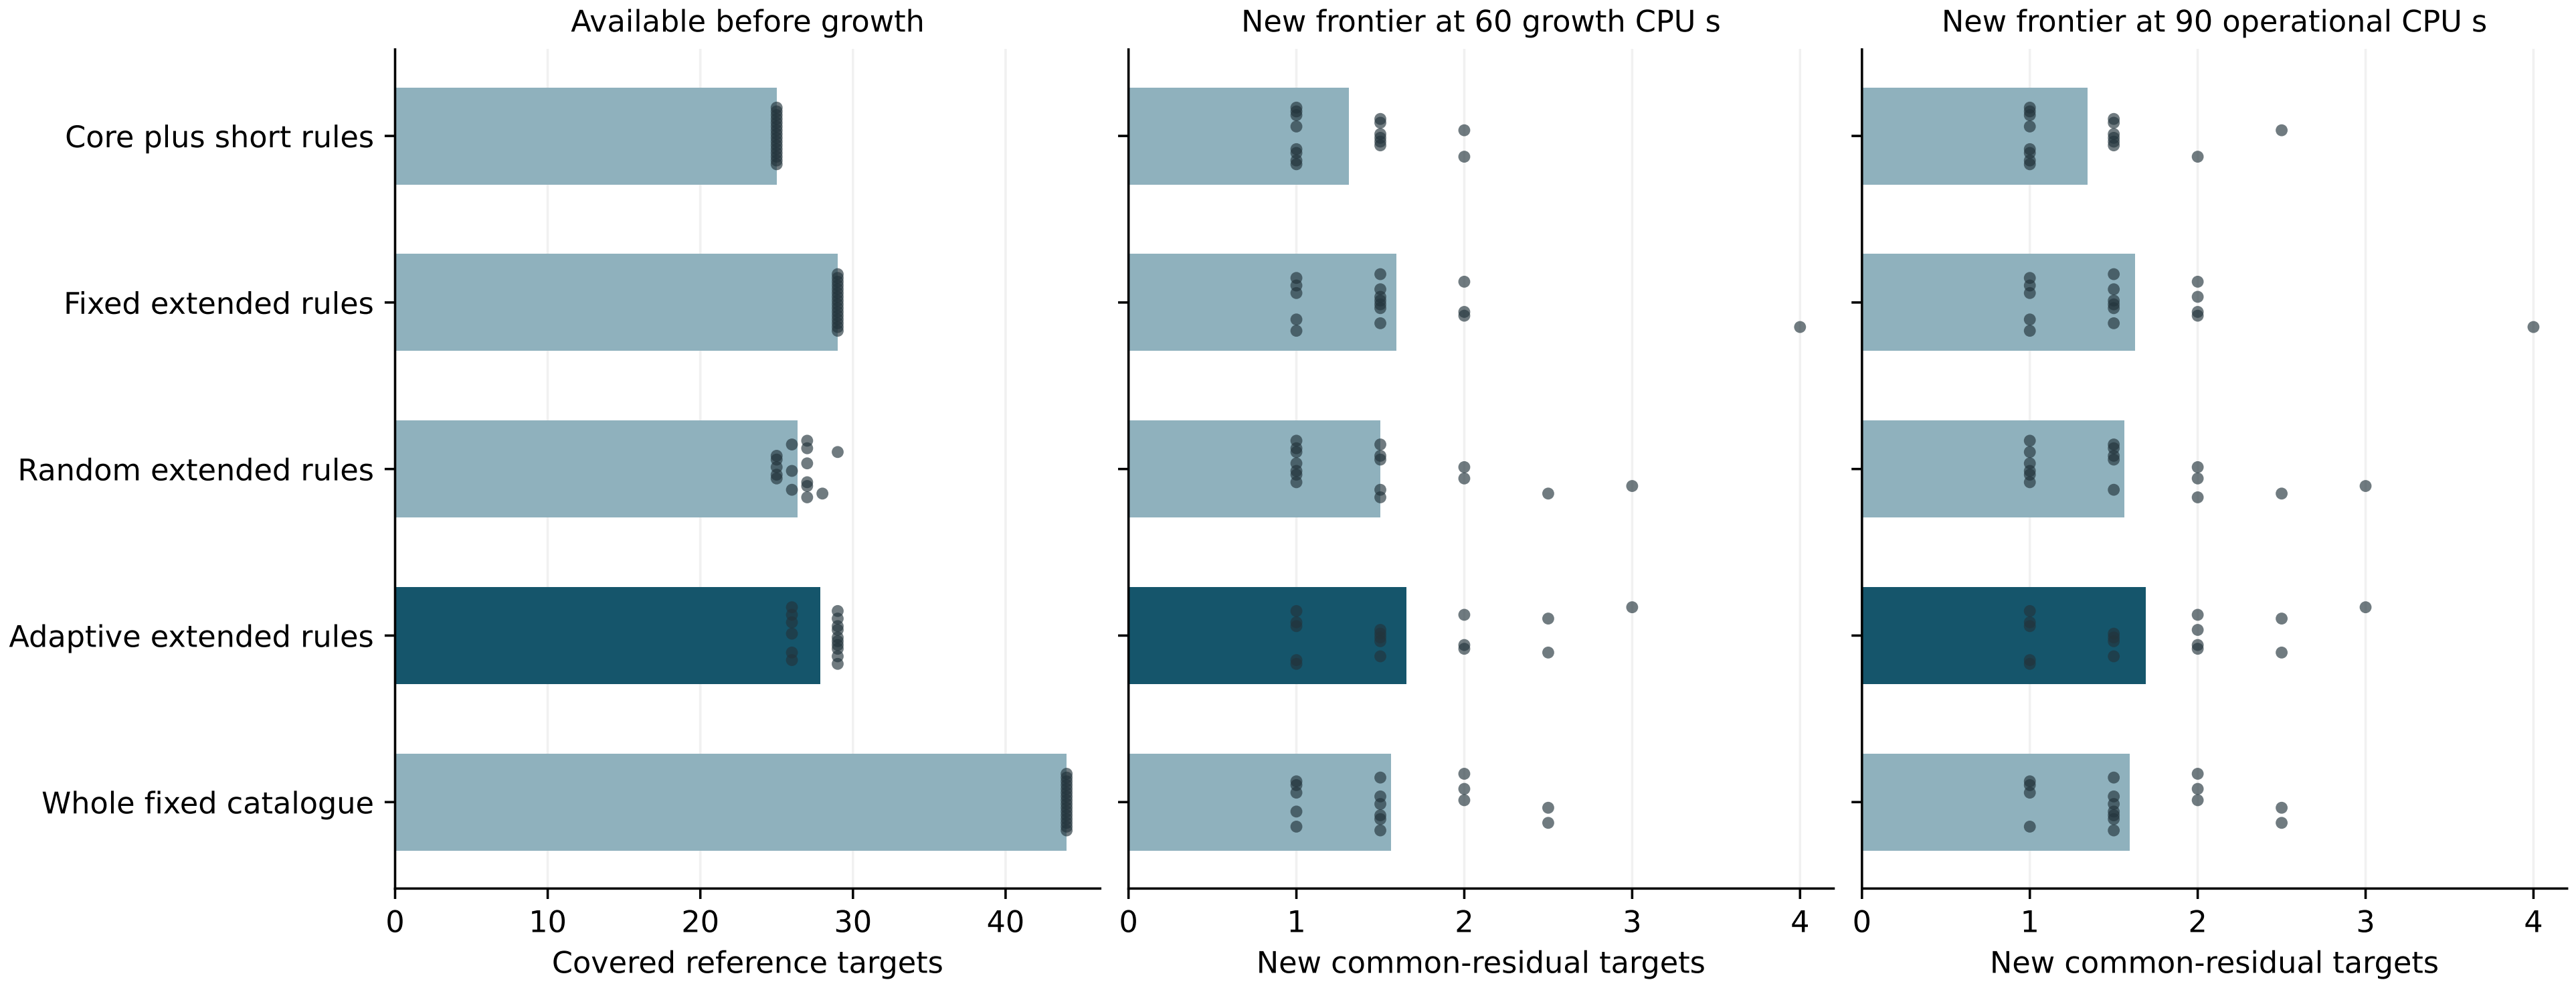
\includegraphics[width=\linewidth,height=.67\textheight,keepaspectratio]{Fig12.png}
\caption{Locked native comparison. Bars represent means over 16 source blocks; dots show source means after averaging the two neutral continuers. Initial coverage counts the whole reference, whereas the future panels count the common initial residual. The figure supplies descriptive variation, not confidence intervals}\label{fig:12}
\end{figure}

The complete registered report remains available in the frozen package, including all arms and paired outcomes. We neither retune on these targets nor infer equivalence from the failed superiority test. The fixed repertoire supplies the working configuration, not a post-hoc claim that it beats every alternative.

\section*{Appendix H. Cumulative skeleton networks}\label{appendix-h.-cumulative-skeleton-networks}
\addcontentsline{toc}{section}{Appendix H. Cumulative skeleton networks}

\subsection*{H.1. Projections and representative choice}\label{h.1.-projections-and-representative-choice}
\addcontentsline{toc}{subsection}{H.1. Projections and representative choice}

The new descriptive study reads only audited initial libraries from the corrected holdout. Each projection includes every available anchor, all 29 basis roots, and every necessary certificate ancestor. The projection joins each parent to the conclusion and collapses duplicate arcs. Hidden ancestors retain proof roles but no automatic search rights. The first source, 2026102201, supplies both representatives. The main text uses its fixed quota-matched control because adaptive ranking failed the registered rule; the image below retains the adaptive representative that we chose before scoring. This editorial fallback does not relabel adaptive as an effective method or select the highest-performing control.

Panels a, c, and d retain their old graph hashes and layouts. Panels c and d also retain their shared coordinates, colours, and vertex areas. Panel b uses the same fixed layout seed, three-start community search, and vertex-area rule. All vertices and unique undirected edges enter every drawing. Layout distances across independently scaled panels do not measure comparable semantic proximity (Fig. S2).

\begin{figure}[!htbp]
\centering
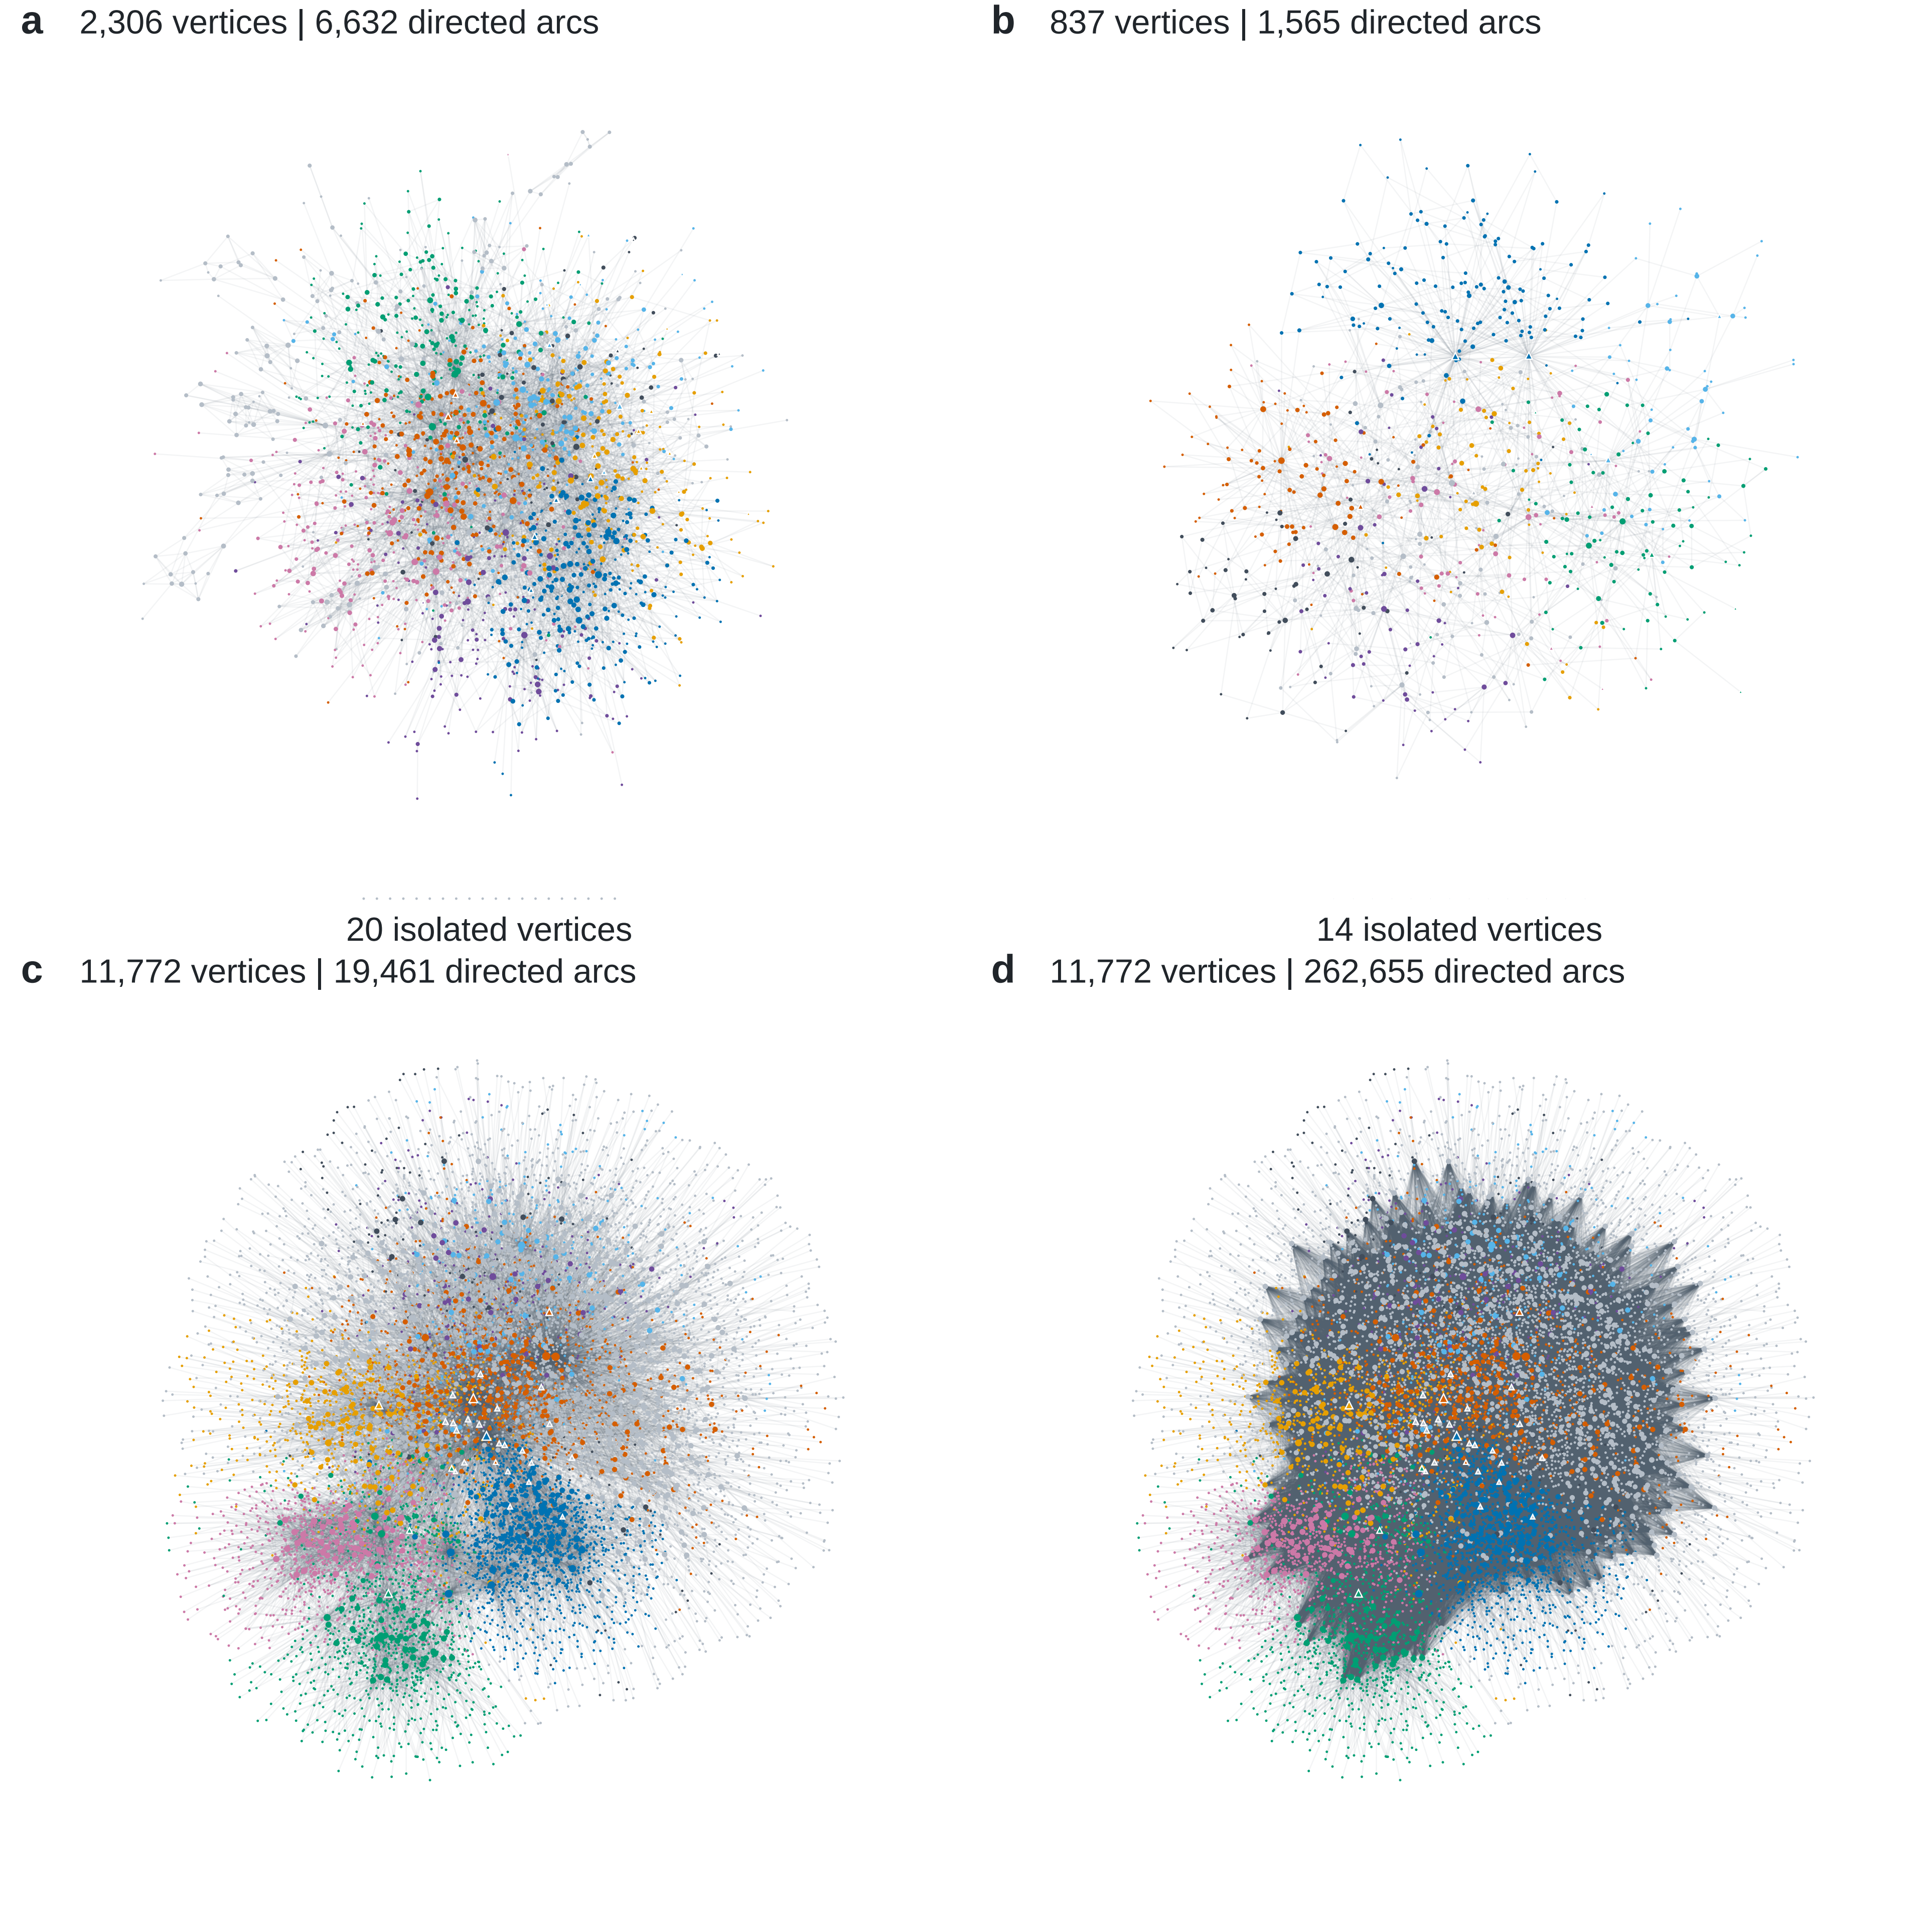
\includegraphics[width=\linewidth,height=.67\textheight,keepaspectratio]{Fig14.png}
\caption{Preselected adaptive test variant on the same basis. Panel b uses adaptive initial source 2026102201, not the best continuation or target-coverage result. The remaining panels retain the frozen Metamath and height-three graphs and layouts. This graph illustrates a tested variant without an established adaptive advantage}\label{fig:14}
\end{figure}

\subsection*{H.2. Profiles across all source states}\label{h.2.-profiles-across-all-source-states}
\addcontentsline{toc}{subsection}{H.2. Profiles across all source states}

Every source contributes one initial library for each of the two reported methods, not two independent theories. Anchors exclude basis roots; certificate vertices include roots and hidden support. C denotes mean local clustering, L the exact mean path on the largest undirected component, Q the best modularity across three Louvain starts, and Q0 the mean over ten simple degree-preserving null graphs. Every new observed and null graph uses all BFS sources.

\subsubsection*{Fixed repertoire}\label{fixed-repertoire}
\addcontentsline{toc}{subsubsection}{Fixed repertoire}

Table S5 reports each fixed-repertoire initial skeleton; source suffixes follow the frozen order.

\begingroup
\small
\setlength{\tabcolsep}{3pt}
\renewcommand{\arraystretch}{1.13}

\begin{longtable}[]{@{}
  >{\raggedright\arraybackslash}p{(\linewidth - 14\tabcolsep) * \real{0.1238}}
  >{\raggedleft\arraybackslash}p{(\linewidth - 14\tabcolsep) * \real{0.1172}}
  >{\raggedleft\arraybackslash}p{(\linewidth - 14\tabcolsep) * \real{0.1732}}
  >{\raggedleft\arraybackslash}p{(\linewidth - 14\tabcolsep) * \real{0.1172}}
  >{\raggedleft\arraybackslash}p{(\linewidth - 14\tabcolsep) * \real{0.1172}}
  >{\raggedleft\arraybackslash}p{(\linewidth - 14\tabcolsep) * \real{0.1172}}
  >{\raggedleft\arraybackslash}p{(\linewidth - 14\tabcolsep) * \real{0.1172}}
  >{\raggedleft\arraybackslash}p{(\linewidth - 14\tabcolsep) * \real{0.1172}}@{}}
\caption{Network profiles of all 16 fixed-repertoire initial skeletons}\label{tab:39}\tabularnewline
\toprule\noalign{}
\begin{minipage}[b]{\linewidth}\raggedright
\textbf{Source suffix}
\end{minipage} & \begin{minipage}[b]{\linewidth}\raggedleft
\textbf{Anchors}
\end{minipage} & \begin{minipage}[b]{\linewidth}\raggedleft
\textbf{Certificate vertices}
\end{minipage} & \begin{minipage}[b]{\linewidth}\raggedleft
\textbf{Arcs}
\end{minipage} & \begin{minipage}[b]{\linewidth}\raggedleft
\textbf{C}
\end{minipage} & \begin{minipage}[b]{\linewidth}\raggedleft
\textbf{L}
\end{minipage} & \begin{minipage}[b]{\linewidth}\raggedleft
\textbf{Q}
\end{minipage} & \begin{minipage}[b]{\linewidth}\raggedleft
\textbf{Q0}
\end{minipage} \\
\midrule\noalign{}
\endfirsthead
\toprule\noalign{}
\begin{minipage}[b]{\linewidth}\raggedright
\textbf{Source suffix}
\end{minipage} & \begin{minipage}[b]{\linewidth}\raggedleft
\textbf{Anchors}
\end{minipage} & \begin{minipage}[b]{\linewidth}\raggedleft
\textbf{Certificate vertices}
\end{minipage} & \begin{minipage}[b]{\linewidth}\raggedleft
\textbf{Arcs}
\end{minipage} & \begin{minipage}[b]{\linewidth}\raggedleft
\textbf{C}
\end{minipage} & \begin{minipage}[b]{\linewidth}\raggedleft
\textbf{L}
\end{minipage} & \begin{minipage}[b]{\linewidth}\raggedleft
\textbf{Q}
\end{minipage} & \begin{minipage}[b]{\linewidth}\raggedleft
\textbf{Q0}
\end{minipage} \\
\midrule\noalign{}
\endhead
\bottomrule\noalign{}
\endlastfoot
01 & 675 & 841 & 1573 & 0.0202 & 4.177 & 0.622 & 0.539 \\
02 & 679 & 852 & 1594 & 0.0199 & 4.179 & 0.622 & 0.542 \\
03 & 665 & 836 & 1564 & 0.0189 & 4.175 & 0.623 & 0.541 \\
04 & 669 & 840 & 1572 & 0.0200 & 4.175 & 0.624 & 0.541 \\
05 & 679 & 847 & 1585 & 0.0200 & 4.167 & 0.623 & 0.541 \\
06 & 669 & 840 & 1571 & 0.0199 & 4.171 & 0.622 & 0.543 \\
07 & 682 & 848 & 1586 & 0.0186 & 4.169 & 0.628 & 0.541 \\
08 & 672 & 844 & 1578 & 0.0207 & 4.179 & 0.623 & 0.541 \\
09 & 674 & 845 & 1583 & 0.0215 & 4.181 & 0.624 & 0.541 \\
10 & 677 & 849 & 1587 & 0.0207 & 4.177 & 0.629 & 0.541 \\
11 & 669 & 840 & 1571 & 0.0188 & 4.183 & 0.625 & 0.540 \\
12 & 674 & 848 & 1589 & 0.0203 & 4.180 & 0.628 & 0.541 \\
13 & 681 & 848 & 1586 & 0.0186 & 4.189 & 0.625 & 0.544 \\
14 & 681 & 849 & 1588 & 0.0207 & 4.165 & 0.624 & 0.540 \\
15 & 672 & 844 & 1579 & 0.0204 & 4.175 & 0.629 & 0.539 \\
16 & 682 & 851 & 1594 & 0.0201 & 4.171 & 0.624 & 0.542 \\
\end{longtable}

\endgroup

Mean anchors: 675.0000; mean certificate vertices: 845.1250; mean modularity: 0.6246.

\subsubsection*{Adaptive test variant}\label{adaptive-test-variant}
\addcontentsline{toc}{subsubsection}{Adaptive test variant}

Table S6 reports the adaptive-test initial skeletons in the same source order.

\begingroup
\small
\setlength{\tabcolsep}{3pt}
\renewcommand{\arraystretch}{1.13}

\begin{longtable}[]{@{}
  >{\raggedright\arraybackslash}p{(\linewidth - 14\tabcolsep) * \real{0.1238}}
  >{\raggedleft\arraybackslash}p{(\linewidth - 14\tabcolsep) * \real{0.1172}}
  >{\raggedleft\arraybackslash}p{(\linewidth - 14\tabcolsep) * \real{0.1732}}
  >{\raggedleft\arraybackslash}p{(\linewidth - 14\tabcolsep) * \real{0.1172}}
  >{\raggedleft\arraybackslash}p{(\linewidth - 14\tabcolsep) * \real{0.1172}}
  >{\raggedleft\arraybackslash}p{(\linewidth - 14\tabcolsep) * \real{0.1172}}
  >{\raggedleft\arraybackslash}p{(\linewidth - 14\tabcolsep) * \real{0.1172}}
  >{\raggedleft\arraybackslash}p{(\linewidth - 14\tabcolsep) * \real{0.1172}}@{}}
\caption{Network profiles of all 16 adaptive-test initial skeletons}\label{tab:40}\tabularnewline
\toprule\noalign{}
\begin{minipage}[b]{\linewidth}\raggedright
\textbf{Source suffix}
\end{minipage} & \begin{minipage}[b]{\linewidth}\raggedleft
\textbf{Anchors}
\end{minipage} & \begin{minipage}[b]{\linewidth}\raggedleft
\textbf{Certificate vertices}
\end{minipage} & \begin{minipage}[b]{\linewidth}\raggedleft
\textbf{Arcs}
\end{minipage} & \begin{minipage}[b]{\linewidth}\raggedleft
\textbf{C}
\end{minipage} & \begin{minipage}[b]{\linewidth}\raggedleft
\textbf{L}
\end{minipage} & \begin{minipage}[b]{\linewidth}\raggedleft
\textbf{Q}
\end{minipage} & \begin{minipage}[b]{\linewidth}\raggedleft
\textbf{Q0}
\end{minipage} \\
\midrule\noalign{}
\endfirsthead
\toprule\noalign{}
\begin{minipage}[b]{\linewidth}\raggedright
\textbf{Source suffix}
\end{minipage} & \begin{minipage}[b]{\linewidth}\raggedleft
\textbf{Anchors}
\end{minipage} & \begin{minipage}[b]{\linewidth}\raggedleft
\textbf{Certificate vertices}
\end{minipage} & \begin{minipage}[b]{\linewidth}\raggedleft
\textbf{Arcs}
\end{minipage} & \begin{minipage}[b]{\linewidth}\raggedleft
\textbf{C}
\end{minipage} & \begin{minipage}[b]{\linewidth}\raggedleft
\textbf{L}
\end{minipage} & \begin{minipage}[b]{\linewidth}\raggedleft
\textbf{Q}
\end{minipage} & \begin{minipage}[b]{\linewidth}\raggedleft
\textbf{Q0}
\end{minipage} \\
\midrule\noalign{}
\endhead
\bottomrule\noalign{}
\endlastfoot
01 & 668 & 837 & 1565 & 0.0197 & 4.170 & 0.631 & 0.541 \\
02 & 679 & 852 & 1594 & 0.0199 & 4.179 & 0.622 & 0.542 \\
03 & 662 & 832 & 1556 & 0.0184 & 4.169 & 0.626 & 0.542 \\
04 & 673 & 843 & 1578 & 0.0185 & 4.160 & 0.624 & 0.541 \\
05 & 672 & 843 & 1577 & 0.0195 & 4.161 & 0.626 & 0.542 \\
06 & 669 & 840 & 1571 & 0.0199 & 4.171 & 0.622 & 0.543 \\
07 & 682 & 848 & 1586 & 0.0186 & 4.169 & 0.628 & 0.541 \\
08 & 669 & 840 & 1570 & 0.0202 & 4.173 & 0.619 & 0.541 \\
09 & 674 & 845 & 1583 & 0.0215 & 4.181 & 0.624 & 0.541 \\
10 & 677 & 849 & 1587 & 0.0207 & 4.177 & 0.629 & 0.541 \\
11 & 669 & 840 & 1571 & 0.0188 & 4.183 & 0.625 & 0.540 \\
12 & 674 & 848 & 1589 & 0.0203 & 4.180 & 0.628 & 0.541 \\
13 & 675 & 846 & 1583 & 0.0181 & 4.182 & 0.619 & 0.542 \\
14 & 681 & 849 & 1588 & 0.0207 & 4.165 & 0.624 & 0.540 \\
15 & 669 & 840 & 1571 & 0.0199 & 4.169 & 0.617 & 0.540 \\
16 & 682 & 851 & 1594 & 0.0201 & 4.171 & 0.624 & 0.542 \\
\end{longtable}

\endgroup

Mean anchors: 673.4375; mean certificate vertices: 843.9375; mean modularity: 0.6243.

\subsection*{H.3. Tail diagnostics and reproducibility}\label{h.3.-tail-diagnostics-and-reproducibility}
\addcontentsline{toc}{subsection}{H.3. Tail diagnostics and reproducibility}

For each outgoing distinct-use profile, the diagnostic uses 20,000 bootstrap draws for the exact discrete pure power-law family and refits the threshold and exponent in every draw. The earlier in-degree and undirected-degree alternatives remain secondary descriptions. Conditional tail diagnostics do not assume independent graph replicates or establish a limiting law. Small-world ratios compare clustering and largest-component paths with ten degree-preserving controls, not a universal classifier.

Across all 16 fixed sources, pure-family bootstrap p-values range from 0.24190 to 0.62575; across the 16 adaptive variants, they range from 0.17950 to 0.62575. None rejects that family at five percent. The new certificate projections retain 13--15 isolated unused basis roots, which still enter the vertex count and zero-degree mass; both illustrated representatives contain 14. A compatible finite tail neither confirms adaptive future-use superiority nor proves that the generator intrinsically converges to a scale-free network. The machine-readable profiles retain thresholds, exponents, binomial Monte Carlo intervals, zero-degree counts, and same-tail alternative likelihoods for every source.

\clearpage
\begin{thebibliography}{37}
\bibitem{FlajoletSedgewick2009} Flajolet, P., \& Sedgewick, R. (2009). \emph{Analytic combinatorics}. Cambridge University Press. \url{https://doi.org/10.1017/CBO9780511801655}

\bibitem{CookReckhow1979} Cook, S. A., \& Reckhow, R. A. (1979). The relative efficiency of propositional proof systems. \emph{Journal of Symbolic Logic}, \emph{44}(1), 36--50. \url{https://doi.org/10.2307/2273702}

\end{thebibliography}
\end{document}
